\chapter{Por qué la placa terminó en 4 capas}\label{cap:capas}

La placa empezó como un diseño de 2 capas y terminó siendo de 4. No fue un capricho ni una decisión tomada al
principio: salió de intentar rutear con unas reglas concretas y comprobar que con 2 capas no había solución sin romper
esas reglas. Para entender por qué esas reglas importan hay que entender primero una idea que casi nunca se explica
bien en los cursos de circuitos: \textbf{la corriente de retorno}.

\textbf{En este capítulo vas a ver:}
\begin{itemize}
  \item qué es la corriente de retorno y por dónde viaja en una placa;
  \item por qué el área del lazo importa (inductancia, acople y emisiones);
  \item qué pasa cuando el plano de tierra tiene un corte debajo de una pista;
  \item por qué los nodos de alta impedancia del canal analógico son tan delicados;
  \item cuál era la regla de 2 capas, qué cruces la hacían imposible y cómo se comprobó;
  \item qué opciones había, por qué se eligió 4 capas y qué se ganó;
  \item el apilado de JLCPCB, el uso de cada capa y cómo se verifica que se respete;
  \item cuánto cuesta y si sigue sirviendo el ensamblaje económico de JLCPCB.
\end{itemize}

% =====================================================================================================
\section{Toda corriente vuelve}\label{sec:c08-vuelve}

En un esquemático dibujas un cable de la salida de un op-amp a la entrada de otro, y la tierra la pones con un
símbolo. Ese símbolo esconde la mitad del circuito. La corriente que sale por la pista tiene que volver a su fuente,
y vuelve \emph{por la tierra}. Siempre hay un lazo cerrado: ida por la pista, vuelta por la tierra.

\begin{idea}[el lazo siempre existe]
Cada señal de la placa forma una espira: la pista de ida y el camino de vuelta por GND. Esa espira tiene un área.
Todo lo malo que le pasa a una señal en una placa (que capte ruido, que meta ruido en otra, que radie) depende de qué
tan grande es esa área. El trabajo del diseñador de la placa es, en buena parte, \textbf{mantener pequeñas las áreas de
los lazos}.
\end{idea}

\begin{figure}[htbp]
\centering
\begin{circuitikz}
  \fill[cobre!15] (0.6,0.3) rectangle (6.4,2.7);
  \node[cobre!70!black,align=center,font=\small] at (3.5,1.5) {área del lazo\\(lo que hay que minimizar)};
  \draw (0,0) to[sV,l=fuente] (0,3) -- (7,3) to[R,l=carga] (7,0);
  \draw[very thick,red!70!black,-{Latex[length=3mm]}] (1.0,3.35) -- (3.0,3.35);
  \node[right,red!70!black,font=\small] at (3.1,3.35) {pista (ida)};
  \draw[very thick,blue!70!black,-{Latex[length=3mm]}] (6.6,-0.35) -- (4.0,-0.35);
  \node[left,blue!70!black,font=\small] at (3.9,-0.35) {retorno por GND (la mitad que no se dibuja)};
  \draw (0,0) -- (7,0);
\end{circuitikz}
\caption{Una señal es una espira: ida por la pista y vuelta por la tierra. El área encerrada es la que capta y emite
ruido.}
\label{fig:c08-lazo}
\end{figure}

% =====================================================================================================
\section{¿Por dónde vuelve la corriente?}\label{sec:c08-donde}

Supón que la pista sale de un punto A, da una vuelta en L y llega a un punto B, y que debajo hay un plano de tierra
entero (una capa de cobre completa). La corriente de retorno tiene muchos caminos posibles por el plano. ¿Cuál toma?

\begin{itemize}
  \item \textbf{A baja frecuencia (DC y muy poca variación)} la corriente se reparte según la \emph{resistencia}: va más o
  menos en línea recta de B a A, abriéndose por todo el plano, porque ese es el camino de menor resistencia.
  \item \textbf{A alta frecuencia} lo que manda es la \emph{inductancia}, no la resistencia. El camino de menor
  inductancia es el que encierra la menor área con la pista de ida, y ese camino es \textbf{justo debajo de la pista}.
  La corriente de retorno se ``pega'' debajo de la pista y la sigue en su vuelta en L.
\end{itemize}

\begin{figure}[htbp]
\centering
\begin{tikzpicture}[scale=0.85]
  % (a) baja frecuencia
  \begin{scope}
    \fill[verdeplaca!12] (0,0) rectangle (6,4);
    \node[above] at (3,4) {\small (a) baja frecuencia: menor resistencia};
    \draw[line width=2.2pt,cobre] (0.8,0.8) -- (5.2,0.8) -- (5.2,3.2);
    \filldraw[fill=white,draw=black] (0.8,0.8) circle (0.12) node[below left]{A};
    \filldraw[fill=white,draw=black] (5.2,3.2) circle (0.12) node[above right]{B};
    \foreach \d in {-0.5,-0.25,0,0.25,0.5}{
      \draw[blue!70!black,-{Latex[length=2mm]},densely dashed] ($(5.2,3.2)+(\d,\d*-0.9)$) .. controls ($(3,2)+(\d*1.6,\d*-1.6)$) .. ($(0.8,0.8)+(\d*0.5,\d*-0.4)$);
    }
    \node[blue!70!black,font=\small,align=center] at (2.2,2.9) {retorno\\repartido};
  \end{scope}
  % (b) alta frecuencia
  \begin{scope}[xshift=7.2cm]
    \fill[verdeplaca!12] (0,0) rectangle (6,4);
    \node[above] at (3,4) {\small (b) alta frecuencia: menor inductancia};
    \draw[line width=9pt,blue!25] (0.8,0.8) -- (5.2,0.8) -- (5.2,3.2);
    \draw[line width=2.2pt,cobre] (0.8,0.8) -- (5.2,0.8) -- (5.2,3.2);
    \draw[blue!70!black,-{Latex[length=2mm]},thick] (5.55,3.0) -- (5.55,1.2);
    \draw[blue!70!black,-{Latex[length=2mm]},thick] (5.0,0.45) -- (1.2,0.45);
    \filldraw[fill=white,draw=black] (0.8,0.8) circle (0.12) node[above left]{A};
    \filldraw[fill=white,draw=black] (5.2,3.2) circle (0.12) node[above right]{B};
    \node[blue!70!black,font=\small,align=center] at (2.6,2.3) {el retorno va\\debajo de la pista};
  \end{scope}
\end{tikzpicture}
\caption{Vista desde arriba de una pista (cobre) sobre un plano de tierra entero (verde). A baja frecuencia el retorno
(azul) toma el camino de menor resistencia; a alta frecuencia se concentra debajo de la pista, que es el lazo de menor
área.}
\label{fig:c08-retorno}
\end{figure}

¿Qué es ``alta frecuencia'' en esta placa? Hay que pensar en los \emph{flancos}, no solo en la frecuencia de repetición.
El nodo de conmutación de los buck (\net{SW_3}, \net{SW_5}) cambia de \SI{0}{\volt} a \SI{24}{\volt} un millón de
veces por segundo, en unos pocos nanosegundos. El reloj de \SI{24.576}{\mega\hertz} del ADC y las líneas I2S
(\net{SAI_SCK}, \net{SAI_FS}, \net{SAI_SD}) también tienen flancos de nanosegundos. Esos flancos tienen contenido
espectral de decenas a cientos de \si{\mega\hertz}, y ahí la corriente de retorno se comporta como en la
figura~\ref{fig:c08-retorno}(b). Hasta el audio, que es lento, se beneficia: la pista de una señal analógica sobre un
plano entero forma un lazo diminuto que casi no capta campo magnético de los vecinos.

\begin{figure}[htbp]
\centering
\begin{tikzpicture}[scale=1.0]
  \fill[green!20!black!8] (0,0) rectangle (9,0.9);
  \node[font=\small] at (7.4,0.45) {prepreg 7628, $\approx$\SI{0.21}{\milli\meter}};
  \fill[verdeplaca!70] (0,-0.12) rectangle (9,0);
  \node[font=\small,anchor=west,text=verdeplaca] at (9.1,-0.06) {\capa{In1.Cu} = GND};
  \fill[cobre] (3.6,0.9) rectangle (4.6,1.07);
  \node[font=\small,anchor=south] at (4.1,1.1) {pista en \capa{F.Cu}};
  \foreach \a in {0.35,0.7,1.1,1.6}{
    \draw[gray,thin] (4.1-\a*0.35,0.9) .. controls (4.1-\a*0.9,0.6) and (4.1-\a*1.3,0.2) .. (4.1-\a*1.4,0);
    \draw[gray,thin] (4.1+\a*0.35,0.9) .. controls (4.1+\a*0.9,0.6) and (4.1+\a*1.3,0.2) .. (4.1+\a*1.4,0);
  }
  \draw[thick] (4.1,0.985) circle (0.07); \fill (4.1,0.985) circle (0.02);
  \foreach \x/\s in {3.5/0.6,3.85/1,4.1/1.3,4.35/1,4.7/0.6}{
    \draw[blue!70!black,line width=\s pt] (\x-0.05,-0.11) -- (\x+0.05,-0.01) (\x-0.05,-0.01) -- (\x+0.05,-0.11);
  }
  \node[font=\small,blue!70!black,anchor=north] at (4.1,-0.2) {retorno concentrado debajo (más denso al centro)};
\end{tikzpicture}
\caption{Corte transversal: la pista de \capa{F.Cu} queda a unos \SI{0.21}{\milli\meter} del plano \capa{In1.Cu}.
El campo (gris) se cierra sobre el plano y la corriente de retorno (cruces azules, entrando a la hoja) se concentra
justo debajo de la pista, que lleva la corriente de ida (punto, saliendo de la hoja).}
\label{fig:c08-corte}
\end{figure}

% =====================================================================================================
\section{Área del lazo: inductancia, acople y emisiones}\label{sec:c08-area}

Un lazo de corriente es, literalmente, una espira. De electromagnetismo recuerdas tres cosas que aplican aquí:

\begin{enumerate}
  \item \textbf{Inductancia.} La inductancia de una espira crece con su área. Si la corriente cambia rápido, aparece
  una tensión $v = L\,\dfrac{di}{dt}$ que no estaba en el esquemático: picos y oscilaciones.
  \item \textbf{Acople (diafonía).} Dos espiras cercanas comparten flujo magnético (inductancia mutua $M$). Lo que pasa
  en una induce $v = M\,\dfrac{di}{dt}$ en la otra. Menos área = menos flujo compartido.
  \item \textbf{Emisiones y susceptibilidad.} Una espira grande es una antena: radia cuando por ella pasa corriente
  rápida y capta campos externos (por ejemplo los \SI{60}{\hertz} de la red o el propio buck).
\end{enumerate}

\begin{calculo}[orden de magnitud del pico en el lazo del buck]
El lazo de entrada del buck (condensador de entrada, pin \net{VIN}, pin \net{PGND}) conmuta la corriente de la bobina
en cada flanco. En el peor caso esa corriente llega a unos \SI{275}{\milli\ampere} \medido{} (pico en
\net{SW_3}/\net{SW_5}, tabla de anchos de \archivo{CALCULOS.md}). Si el flanco dura unos \SI{10}{\nano\second}
\estimado{} (el mismo supuesto de \archivo{CALCULOS.md}):
\[
\frac{di}{dt} \approx \frac{\SI{0.275}{\ampere}}{\SI{10}{\nano\second}} = \SI{27.5}{\mega\ampere\per\second}.
\]
Con apenas \SI{1}{\nano\henry} de inductancia parásita en el lazo \estimado{}:
\[
v = L\,\frac{di}{dt} = \SI{1}{\nano\henry}\times\SI{27.5}{\mega\ampere\per\second} \approx \SI{28}{\milli\volt}
\]
en cada flanco, un millón de veces por segundo. Si el lazo fuera diez veces más grande, el pico sería unas diez veces
mayor. Por eso el lazo VIN--CHF--PGND del buck se dibujó lo más chico posible (capítulo~\ref{cap:ruteo}): mide
\SI{7.25}{\milli\meter} de perímetro y \SI{3.32}{\milli\meter\squared} de área en un lado del integrado
\medido{}.
\end{calculo}

% =====================================================================================================
\section{Qué pasa si el plano tiene un corte}\label{sec:c08-ranura}

Ahora imagina que debajo de la pista el plano tiene un corte (una ranura). Puede ser porque otra pista pasa por esa
capa, porque hay una fila de vías con sus holguras unidas, o porque alguien partió el plano en ``tierra analógica'' y
``tierra digital''. La corriente de retorno de alta frecuencia quería ir justo debajo de la pista, pero ahí no hay
cobre: tiene que \textbf{rodear la ranura}.

\begin{figure}[htbp]
\centering
\begin{tikzpicture}[scale=0.95]
  \fill[verdeplaca!12] (0,0) rectangle (10,4);
  \fill[white] (4.4,0.9) rectangle (5.6,4);
  \draw[gray] (4.4,0.9) rectangle (5.6,4);
  \node[font=\small,gray!50!black,anchor=south] at (5,4.05) {ranura en el plano};
  \fill[rojoojo!20] (4.2,2) rectangle (5.8,0.6);
  \draw[line width=2.4pt,cobre] (1,2) -- (9,2);
  \node[above,font=\small] at (2.6,2.05) {pista (ida)};
  \draw[blue!70!black,thick,-{Latex[length=2.2mm]}] (9,1.8) -- (5.8,1.8) -- (5.8,0.6) -- (4.2,0.6) -- (4.2,1.8) -- (1.2,1.8);
  \node[font=\small,blue!70!black,align=left,anchor=west] at (6.0,1.05) {el retorno tiene\\que rodear la ranura};
  \node[font=\small,rojoojo,anchor=north] at (5,0.5) {área extra del lazo};
  \filldraw[fill=white] (1,2) circle (0.1); \filldraw[fill=white] (9,2) circle (0.1);
\end{tikzpicture}
\caption{Una ranura en el plano obliga a la corriente de retorno a rodearla. El lazo crece (rojo): más inductancia,
más acople y la ranura misma se comporta como una antena.}
\label{fig:c08-ranura}
\end{figure}

Las consecuencias son las de la sección anterior, pero peores: el lazo crece justo donde está la ranura, y la ranura
pone en el mismo camino de retorno a todas las señales que la cruzan, así que se acoplan entre ellas. Por eso la nota
de TI SLYT499 pide \textbf{un solo plano de tierra, sin cortes ni ranuras bajo las pistas}, y advierte que hasta las
holguras de las vías pueden formar ranuras si se alinean \doc{SLYT499 p.8}. Y la nota SLYT512 explica cómo ordenar una
placa con convertidor: un solo plano, \emph{repartido por zonas} (lo analógico se rutea sobre su zona y lo digital
sobre la suya) en lugar de partido \doc{SLYT512 pp.5--6}.

\begin{ojo}[una pista en el plano también es una ranura]
En una placa de 2 capas en la que \capa{B.Cu} hace de plano, \textbf{cada pista que pongas en \capa{B.Cu} corta el
plano}. El relleno de tierra se aparta de la pista dejando una franja sin cobre: eso es una ranura. Si encima de esa
franja pasa una señal sensible en \capa{F.Cu}, su retorno tiene que rodear. Esta es la raíz de todo el problema de las
2 capas.
\end{ojo}

% =====================================================================================================
\section{Por qué los nodos de alta impedancia son delicados}\label{sec:c08-altaz}

El canal analógico tiene nodos de impedancia muy alta: la cadena de \SI{1}{\mega\ohm} que baja la señal del micrófono
(\net{R13}, \net{R14}, \net{R16}, \net{R18}, capítulo~\ref{cap:analog}), el nodo filtrado del DAC (\net{DAC_F}) y el
nodo medio de la realimentación (\net{FB_MID}). En esos nodos un acople capacitivo pequeño basta para meter ruido.

\begin{calculo}[acople capacitivo en un nodo de la cadena de 1 M$\Omega$]
Toma el nodo \net{IEPE_DIV1}, entre \net{R13} (\SI{390}{\kilo\ohm}) y \net{R14} (\SI{365}{\kilo\ohm}). Hacia
la derecha la cadena sigue con \SI{191}{\kilo\ohm} y \SI{54.9}{\kilo\ohm} hasta el nodo \net{SUM}, que es una tierra
virtual del op-amp, y hacia la izquierda está la salida del micrófono, de baja impedancia. La impedancia que ``ve''
ese nodo es el paralelo:
\[
R_\text{th} = \SI{390}{\kilo\ohm} \parallel (\num{365}+\num{191}+\num{54.9})\,\si{\kilo\ohm}
= \SI{390}{\kilo\ohm} \parallel \SI{610.9}{\kilo\ohm} \approx \SI{238}{\kilo\ohm}.
\]
Supón que una pista ruidosa pasa cerca y forma con el nodo una capacidad parásita de solo \SI{0.1}{\pico\farad}
\estimado{}. Para la componente de \SI{1}{\mega\hertz} del buck:
\[
X_C = \frac{1}{2\pi f C} = \frac{1}{2\pi\cdot\SI{1}{\mega\hertz}\cdot\SI{0.1}{\pico\farad}} \approx \SI{1.59}{\mega\ohm}.
\]
El acople es un divisor entre $X_C$ y $R_\text{th}$:
\[
\frac{|v_\text{nodo}|}{|v_\text{ruido}|} = \frac{R_\text{th}}{\sqrt{R_\text{th}^2 + X_C^2}}
= \frac{238}{\sqrt{238^2+1590^2}} \approx \num{0.15}.
\]
¡Un 15\,\% del ruido pasa al nodo! Si el mismo acople fuera sobre un nodo de \SI{50}{\ohm} (la salida de un op-amp o
de un micrófono IEPE), la relación sería $50/1.59\times10^{6} \approx \num{3e-5}$. Por eso la regla es estricta con
estos nodos: nada ruidoso cerca, y nada que pase por debajo en otra capa.
\end{calculo}

% =====================================================================================================
\section{La regla original para 2 capas}\label{sec:c08-regla2}

Con todo lo anterior, esta fue la regla de ruteo que se aprobó al principio para una placa de 2 capas (punto de
control 2, sección 1 de \archivo{PLAN_RUTEO.md}):

\begin{itemize}
  \item \capa{B.Cu} es el plano de tierra, lo más entero posible.
  \item Las señales críticas (relojes, nodos \net{SW}, \net{IEPE}, \net{SUM}, la cadena de \SI{1}{\mega\ohm},
  \net{REST}, entradas del ADC, \net{VREF}, salidas filtradas de los DAC) van \textbf{100\,\% en \capa{F.Cu}} y
  \textbf{nunca encima de una pista de \capa{B.Cu}}.
  \item Solo I2C, \net{DC_MON} y \net{DC_MON2} (señales lentas o de DC) pueden bajar a \capa{B.Cu}, en puentes
  cortos (\SI{5}{\milli\meter} o menos), con vías de cosido en los extremos y \textbf{solo en la zona digital} (del
  lado de la NUCLEO, $x \geq \SI{70}{\milli\meter}$).
  \item Los cruces que quedaran se resolvían por topología o pasando por debajo de una resistencia o condensador 0603
  en la misma capa (entre los dos pads de un 0603 quedan \SI{0.85}{\milli\meter} libres, y cabe una pista de
  \SI{0.2}{\milli\meter} con su separación).
\end{itemize}

Más adelante se aprobaron tres puentes cortos en \capa{B.Cu} debajo del bus de \SI{24}{\volt} (el tronco de
\net{3V3} y los sensados de realimentación de los dos buck), porque ahí solo se cruzan redes de potencia entre sí.

% =====================================================================================================
\section{Por qué no tenía solución}\label{sec:c08-sinsolucion}

\subsection{Los cruces inevitables}

Un cruce es inevitable cuando dos redes tienen que conectar puntos que quedan ``del otro lado'' de la otra. Piénsalo
como dos caminos en un mapa: si la red A tiene que unir dos puntos y la red B, junto con las piezas que conecta, forma
una barrera cerrada entre ellos, A no puede llegar sin cruzar B. En una sola capa eso no tiene arreglo; o pasas por
debajo de una pieza (si la red B tiene una pieza en serie con espacio entre pads), o cambias de capa.

\begin{figure}[htbp]
\centering
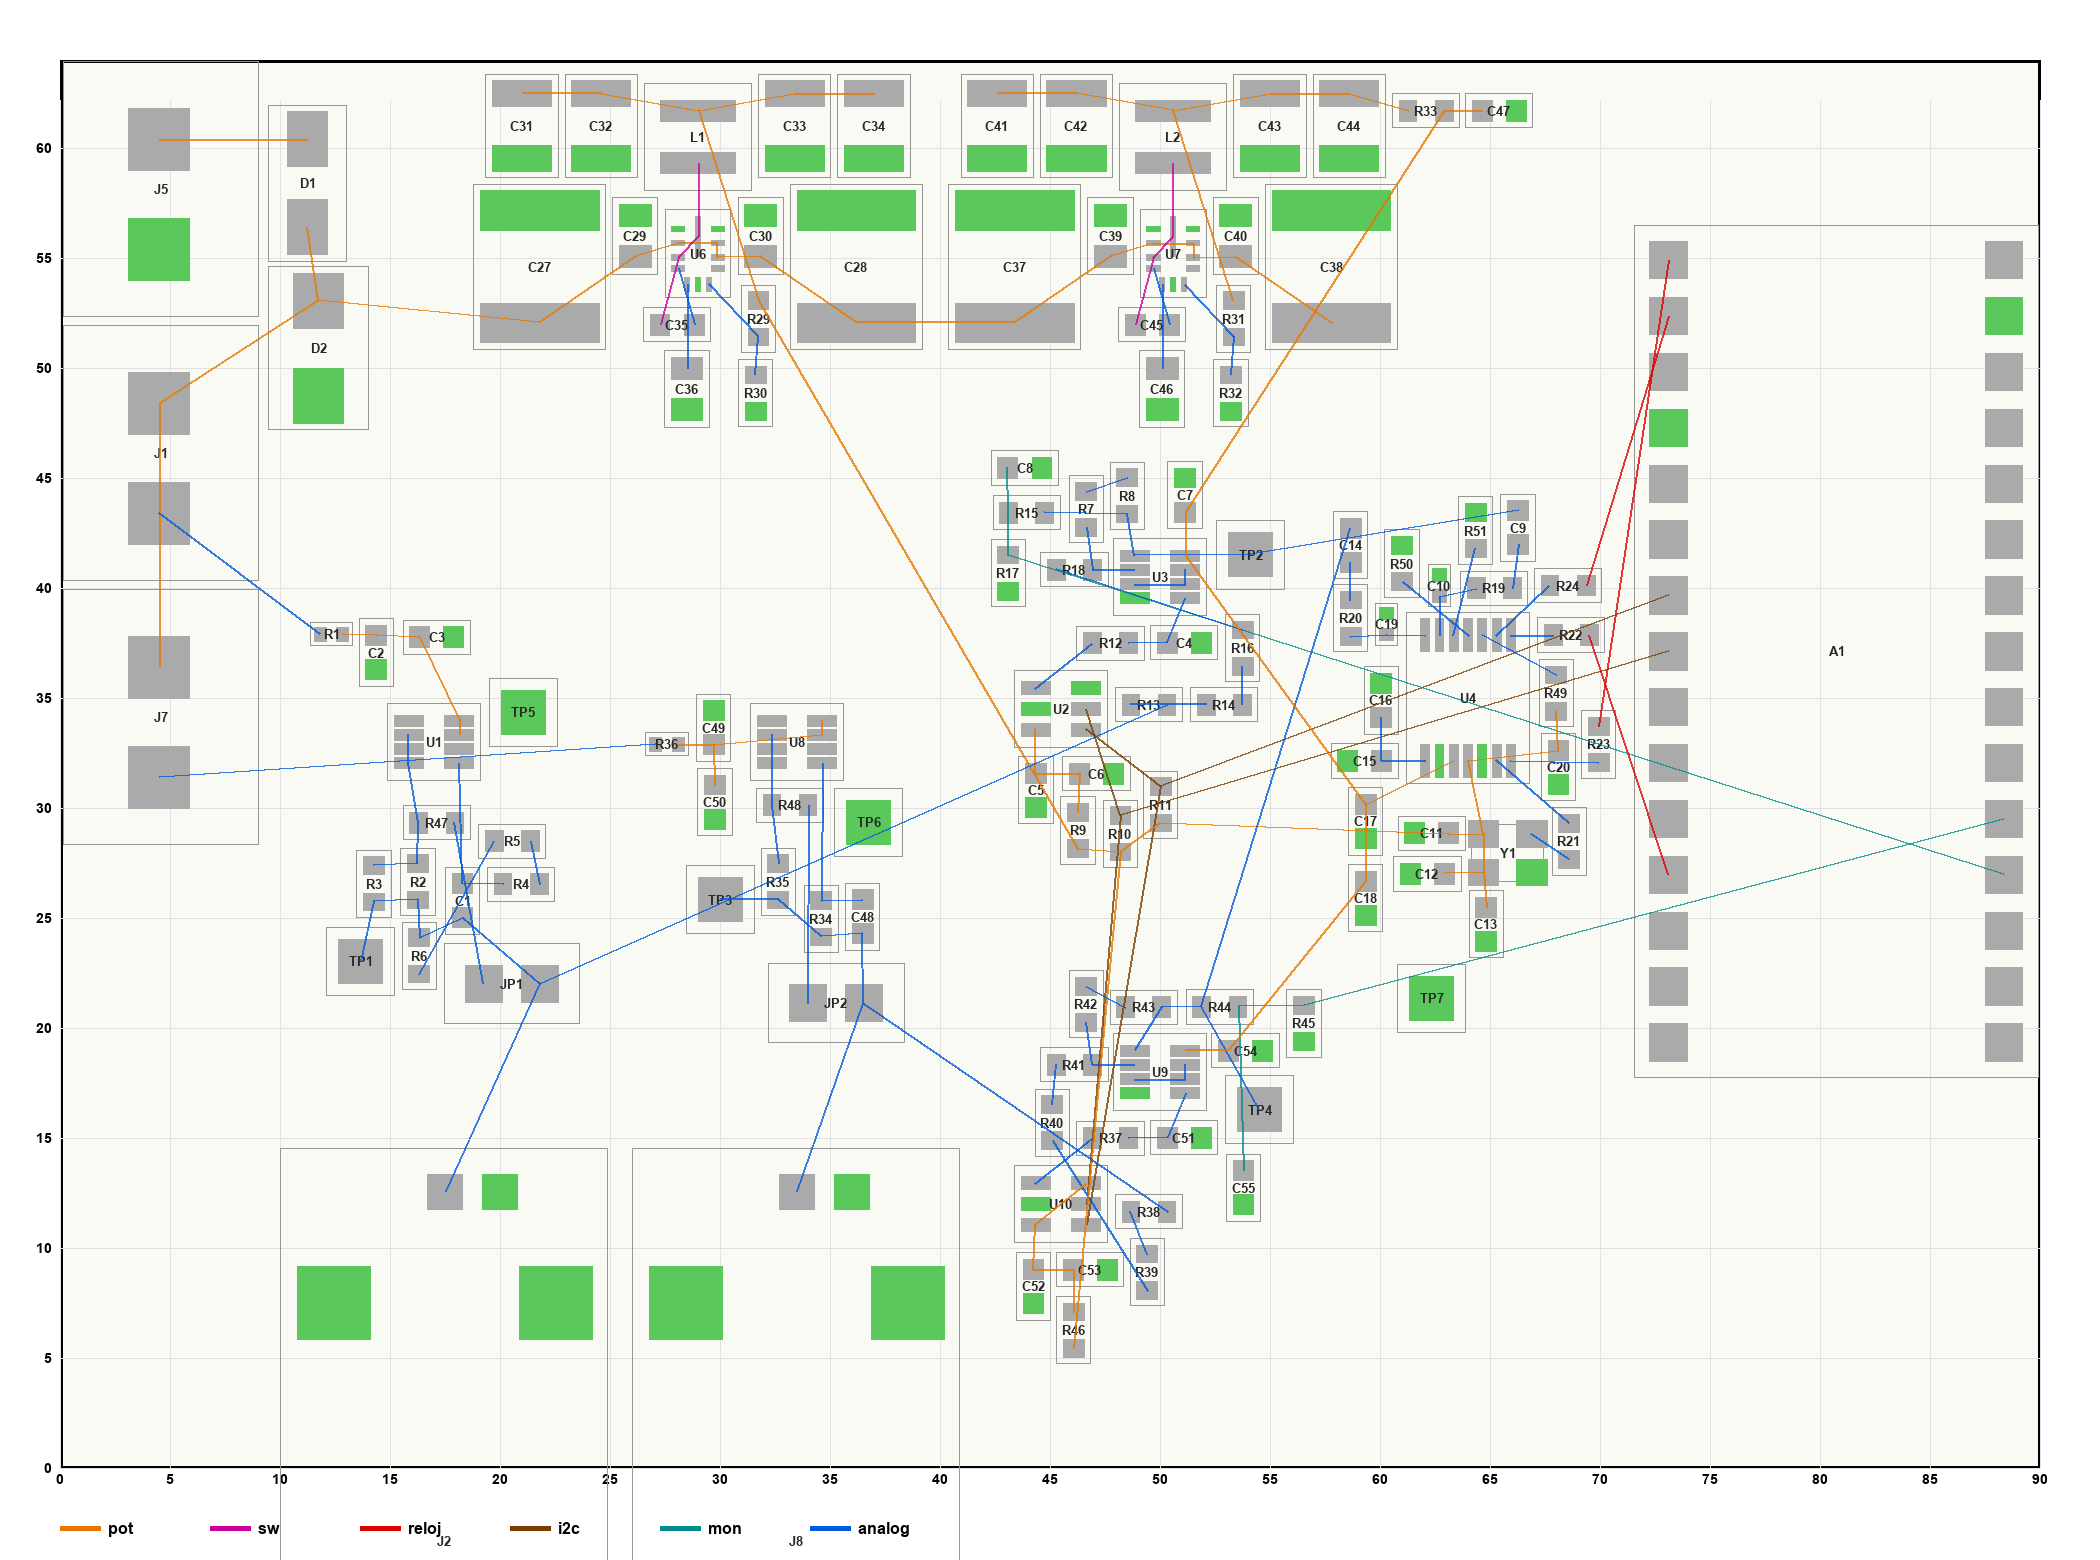
\includegraphics[width=\linewidth]{figuras/c08_ratsnest.png}
\caption{Mapa de las conexiones pendientes antes de rutear (``ratsnest'') sobre el placement, sin GND. Coordenadas en
mm desde la esquina inferior izquierda. Colores: potencia (naranja), nodos SW (magenta), reloj (rojo), I2C (marrón),
\net{DC_MON} (verde azulado) y analógicas (azul). Fíjate en las líneas marrones del I2C y las verde azuladas de
\net{DC_MON}: nacen en los AFE, al centro, y tienen que llegar a la NUCLEO (\net{A1}), a la derecha, atravesando el ADC y
las líneas azules que bajan.}
\label{fig:c08-ratsnest}
\end{figure}

Con el placement real, el análisis a mano encontró estos cruces (\archivo{PLAN_RUTEO.md}~§1.1):

\begin{center}
\begin{tabularx}{\linewidth}{@{}L{0.21\linewidth}Y@{}}
\toprule
\textbf{Cruce} & \textbf{Por qué no se evita en una capa} \\
\midrule
\net{3V3} × \net{24V_PROT} & El buck de \SI{3.3}{\volt} (\net{U6}) queda encerrado por la entrada
(\net{J5}--\net{D1}--\net{D2}), los condensadores de entrada, el bus de \SI{24}{\volt} hacia \net{U7} y el borde
superior. El bus de \SI{24}{\volt} no tiene una pieza en serie bajo la que pasar. \\
\net{5V_A} × \net{REST_OUT} & \net{5V_A} llega a \net{U3} (pin 8, condensador \net{C7}) por la derecha y
\net{REST_OUT} sale de \net{U3} (pin 1) también hacia la derecha: tiene que cruzar el enlace \net{C7}--\net{U3.8}. \\
\net{5V_A} × \net{REST_SV} & \net{REST_SV} sube de \net{U9} a \net{C14} entre el AFE y el ADC; \net{5V_A} tiene que
llegar a \net{U9} y \net{U3}, que quedan del otro lado. \\
I2C × redes del AFE & Los DAC \net{U2} y \net{U10} están dentro de los AFE, rodeados por \net{REST}, la cadena de
\SI{1}{\mega\ohm} y \net{5V_A}. \\
\bottomrule
\end{tabularx}
\end{center}

\subsection{El ``oráculo'': usar un autorouter para preguntar si hay solución}

Para no depender solo de razonamientos a mano, se usó Freerouting (un autorouter libre) sobre \emph{copias} de la
placa, como herramienta de factibilidad. La idea: si un autorouter, que prueba miles de caminos, no encuentra solución
con una regla, es una señal fuerte de que no la hay. A eso se le llamó el \textbf{oráculo}. Lo que sale del oráculo
\emph{nunca} se copió a la placa: el ruteo real se hizo a mano (capítulo~\ref{cap:ruteo}).

\begin{ojo}[un primer intento que no probaba nada]
La primera corrida de Freerouting bajó de 74 a 32--36 conexiones sin rutear y se estancó. Ese número se trató como
\textbf{indicio, no prueba}: no se guardó el resultado, usaba los pads viejos del TSOT, anchos de \SI{0.5}{\milli\meter}
en pines de paso \SIrange{0.5}{0.65}{\milli\meter} (fallas que podían ser de acceso a pines y no de cruces), no hubo
corrida de control y el límite de pasadas estaba mal configurado. Se rehízo bien, por etapas, en copias.
\end{ojo}

\textbf{Etapa 1, solo las redes críticas} (analógicas y relojes de los bloques 4--7, todo en \capa{F.Cu}). Con el
placement original quedaba sin rutear el AFE del canal 1 en dos enlaces (\net{IEPE}~$\to$~\net{R13.2} y el final de
la cadena, \net{R16}~$\to$~\net{R18}): \net{U3} quedaba encerrado por sus propias redes. Se propuso poner
\net{R13}, \net{R14} y \net{R16} en una columna vertical libre ($x = \num{140.6}$ en coordenadas de KiCad) y con eso \textbf{todas las redes críticas
salieron en \capa{F.Cu} sin una sola vía}. Ese cambio de placement se aprobó (capítulo~\ref{cap:placement}).

\textbf{Etapa 2, el resto} (alimentación, I2C, \net{DC_MON}, straps), con las críticas ya fijas:

\begin{center}
\begin{tabularx}{\linewidth}{@{}L{0.27\linewidth}YL{0.16\linewidth}@{}}
\toprule
\textbf{Corrida} & \textbf{Uso de \capa{B.Cu}} & \textbf{Sin rutear} \\
\midrule
\capa{B.Cu} libre para esas redes & unos \SI{140}{\milli\meter} en 7 tramos, debajo de unas 12 redes críticas
(\net{REST_SV}, \net{SAI_FS}, \net{SAI_SCK}, \net{DOUT}, \net{VINL}, \net{AC_RIGHT}, \net{VSHIFT}, \net{REST_OUT}…) & 3 \\
Vías penalizadas & I2C casi entero en \capa{B.Cu}, unos \SI{37}{\milli\meter} por línea & 17 \\
\bottomrule
\end{tabularx}
\end{center}

\begin{figure}[htbp]
\centering
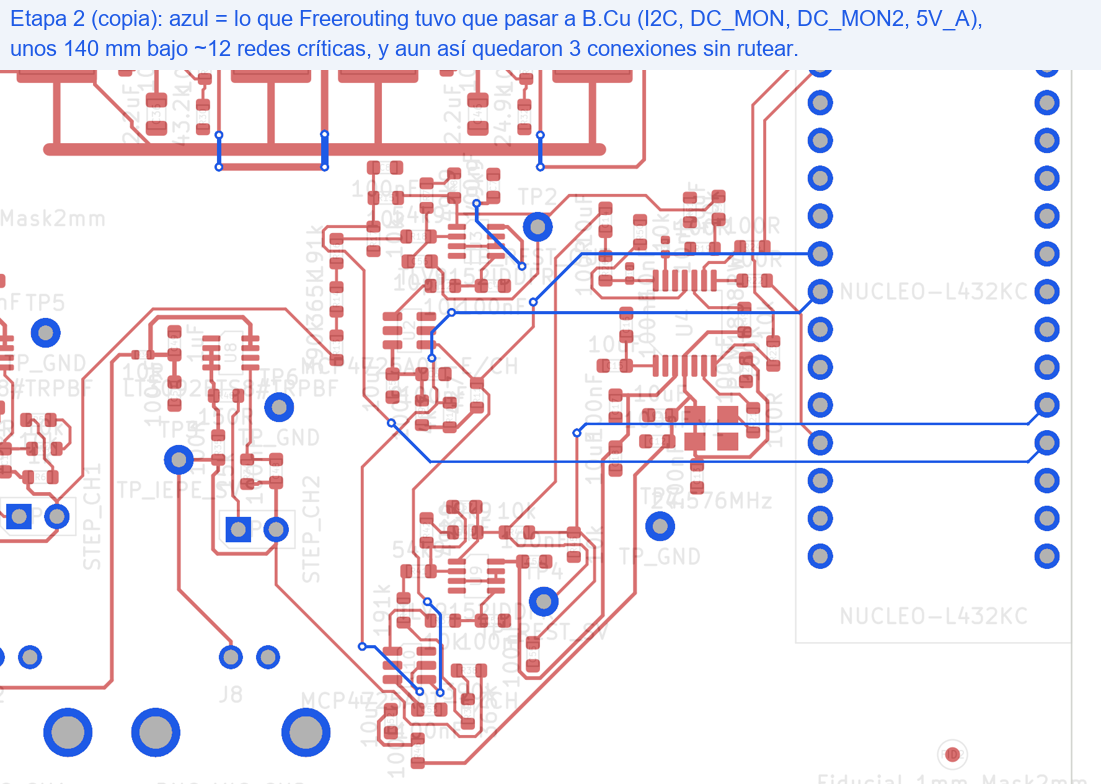
\includegraphics[width=0.92\linewidth]{figuras/oraculo_etapa2_bcu.png}
\caption{Oráculo, etapa 2 (copia de la placa): en azul lo que Freerouting tuvo que pasar a \capa{B.Cu} (I2C,
\net{DC_MON}, \net{DC_MON2}, \net{5V_A}). Son unos \SI{140}{\milli\meter} que cortan el plano debajo de unas 12 redes
críticas, y aun así quedaron 3 conexiones sin rutear.}
\label{fig:c08-oraculo}
\end{figure}

\subsection{La causa de fondo}

No era mala suerte con un par de pistas. Es la estructura del circuito sobre esta placa:
\begin{itemize}
  \item I2C, \net{DC_MON} y \net{DC_MON2} \textbf{nacen dentro de los dos AFE} (en el centro de la placa) y tienen que
  ir a la NUCLEO (a la derecha).
  \item Entre medio, las entradas del ADC y \net{REST_SV} bajan de arriba abajo: son una ``pared'' de señales críticas.
  \item \net{5V_A} y \net{3V3} salen de los buck (arriba) y tienen que entrar a grupos cerrados: \net{U3.8},
  \net{U9.8}, \net{U4.3}, el grupo de \net{3V3} del ADC y \net{C20}/\net{R49}.
\end{itemize}
Con la regla aprobada, cada una de esas redes lentas tendría que cruzar la pared por \capa{B.Cu}, debajo de señales
críticas y fuera de la zona digital, que es justo lo que la regla prohibía.

% =====================================================================================================
\section{Las opciones y la decisión}\label{sec:c08-opciones}

\begin{center}
\begin{tabularx}{\linewidth}{@{}L{0.17\linewidth}YY@{}}
\toprule
\textbf{Opción} & \textbf{Qué implica} & \textbf{Pros y contras} \\
\midrule
A: 2 capas con puentes cortos & Puentes de \SI{3}{\milli\meter} o menos, a \ang{90}, solo de rieles filtrados, I2C o redes
estáticas, y solo bajo señales de baja impedancia. & Más barata. Pero el ruteo es lento (cada puente se diseña y
justifica) y la etapa 2 mostró que no alcanzaba con puentes cortos. \\
A$'$: 2 capas con excepciones & Tramos largos de \capa{B.Cu} debajo de redes críticas (lo que hizo el oráculo). &
Rompe la regla justo en las señales que más la necesitan. \\
B: 4 capas & \capa{In1.Cu} plano GND entero; \capa{In2.Cu} alimentación y señales lentas; \capa{B.Cu} GND y señales
lentas. & Cumple la regla \textbf{sin excepciones de cruce}; no cambia placement ni esquemático; los bloques 1--3 ya
ruteados siguen valiendo. Cuesta más la placa desnuda. \\
C: recolocar la mitad derecha & Mover bloques enteros para que las redes no se crucen. & Cambio grande de placement
y sin garantía de solución. No se recomendó. \\
\bottomrule
\end{tabularx}
\end{center}

\begin{decision}[pasar a 4 capas (opción B)]
\textbf{Qué se decidió:} placa de 4 capas con el apilado estándar de JLCPCB (commit \texttt{3ccda8e}).

\textbf{Alternativas:} 2 capas con puentes (A), 2 capas con excepciones (A$'$) o recolocar bloques (C).

\textbf{Por qué:}
\begin{itemize}
  \item Con 2 capas la regla de cruces no tenía solución con el placement real (análisis a mano + oráculo).
  \item Con 4 capas, \capa{In1.Cu} es un plano GND \emph{entero} a \SI{0.21}{\milli\meter} debajo de todas las pistas
  de \capa{F.Cu}: cada señal crítica tiene su retorno justo debajo, y las redes lentas se cruzan por \capa{In2.Cu} y
  \capa{B.Cu} sin cortar ese plano.
  \item Es lo que hacen los diseños de referencia del fabricante: las placas de evaluación de TI del LMR36015 y del
  PCM1808 son de 4 capas \doc{REGLAS.md §6}, y el propio datasheet del LMR36015 une los dos pines \net{VIN} por una capa
  interna \doc{SNVSB49D fig.~12-2}.
  \item No obliga a tocar el placement ni el esquemático, y lo ruteado en los bloques 1--3 se conservó.
\end{itemize}

\textbf{Fuente:} \archivo{PLAN_RUTEO.md} §1, §2, §10 y §10.1.
\end{decision}

Lo que se ganó, en concreto: \textbf{cero excepciones a la regla de cruces}. Las únicas pistas que pasan por debajo
de otras son señales lentas en \capa{In2.Cu} y \capa{B.Cu}, y una herramienta comprueba que ninguna pase debajo de un
nodo protegido (sección~\ref{sec:c08-politica}).

% =====================================================================================================
\section{El apilado JLC04161H-7628}\label{sec:c08-apilado}

``Apilado'' (\emph{stackup}) es cómo están ordenadas y separadas las capas de cobre dentro de la placa. JLCPCB tiene
apilados estándar; para 4 capas y \SI{1.6}{\milli\meter} el que se usó es el JLC04161H-7628. El ensamblaje económico
de JLCPCB solo acepta apilados estándar \doc{página de capacidades PCBA}.

\begin{figure}[htbp]
\centering
\begin{tikzpicture}[yscale=6,xscale=1]
  % de abajo hacia arriba, en mm
  \def\cu{0.035}\def\pp{0.2104}\def\inn{0.0152}\def\core{1.065}
  \pgfmathsetmacro{\yA}{0}
  \pgfmathsetmacro{\yB}{\cu}
  \pgfmathsetmacro{\yC}{\cu+\pp}
  \pgfmathsetmacro{\yD}{\cu+\pp+\inn}
  \pgfmathsetmacro{\yE}{\cu+\pp+\inn+\core}
  \pgfmathsetmacro{\yF}{\cu+\pp+2*\inn+\core}
  \pgfmathsetmacro{\yG}{\cu+2*\pp+2*\inn+\core}
  \pgfmathsetmacro{\yH}{2*\cu+2*\pp+2*\inn+\core}
  \fill[cobre] (0,\yA) rectangle (4.5,\yB);
  \fill[green!25!black!12] (0,\yB) rectangle (4.5,\yC);
  \fill[orange!80!black] (0,\yC) rectangle (4.5,\yD);
  \fill[green!25!black!20] (0,\yD) rectangle (4.5,\yE);
  \fill[verdeplaca!80] (0,\yE) rectangle (4.5,\yF);
  \fill[green!25!black!12] (0,\yF) rectangle (4.5,\yG);
  \fill[cobre] (0,\yG) rectangle (4.5,\yH);
  \node[anchor=west,font=\footnotesize] at (4.7,\yH-0.0175) {\capa{F.Cu} \SI{0.035}{\milli\meter} (1 oz): piezas y señales críticas};
  \node[anchor=west,font=\footnotesize] at (4.7,\yF/2+\yG/2) {prepreg 7628 \SI{0.2104}{\milli\meter}, $\varepsilon_r \approx \num{4.4}$};
  \node[anchor=west,font=\footnotesize] at (4.7,\yF+0.02) {\capa{In1.Cu} \SI{0.0152}{\milli\meter}: GND entero};
  \node[anchor=west,font=\footnotesize] at (4.7,\yD/2+\yE/2) {núcleo \SI{1.065}{\milli\meter}, $\varepsilon_r \approx \num{4.6}$};
  \node[anchor=west,font=\footnotesize] at (4.7,\yD-0.02) {\capa{In2.Cu} \SI{0.0152}{\milli\meter}: alimentación y lentas};
  \node[anchor=west,font=\footnotesize] at (4.7,\yB/2+\yC/2) {prepreg 7628 \SI{0.2104}{\milli\meter}};
  \node[anchor=west,font=\footnotesize] at (4.7,\yA+0.0175) {\capa{B.Cu} \SI{0.035}{\milli\meter} (1 oz): GND y lentas};
  \draw[|-|] (-0.3,\yA) -- node[left,font=\small]{$\approx$\SI{1.6}{\milli\meter}} (-0.3,\yH);
\end{tikzpicture}
\caption{Apilado JLC04161H-7628 dibujado a escala vertical (los cobres internos son tan finos que casi no se ven).
Espesores y permitividades de la página de impedancia de JLCPCB \doc{REGLAS.md §9}. Fíjate que \capa{In1.Cu} está muy
cerca de \capa{F.Cu} (un prepreg) y lejos de \capa{In2.Cu} (el núcleo).}
\label{fig:c08-apilado}
\end{figure}

Lo más importante del dibujo es la distancia de \capa{F.Cu} a \capa{In1.Cu}: \SI{0.2104}{\milli\meter}. Cuanto más
cerca está el plano, más pegado va el retorno debajo de la pista y más chico es el lazo (figura~\ref{fig:c08-corte}).
En 2 capas, el plano (\capa{B.Cu}) habría quedado al otro lado de toda la placa, a casi \SI{1.5}{\milli\meter}
\estimado{}. Por eso las señales críticas van en
\capa{F.Cu}, la capa que tiene el plano más cerca.

\subsection{Para qué se usa cada capa}

\begin{center}
\begin{tabularx}{\linewidth}{@{}L{0.14\linewidth}YL{0.2\linewidth}@{}}
\toprule
\textbf{Capa} & \textbf{Uso} & \textbf{Pistas \medido} \\
\midrule
\capa{F.Cu} & Piezas y todas las redes críticas; relleno GND cosido en lo que queda libre; zonas de
\SI{24}{\volt}, \net{SW} y salidas de los buck. & \SI{925}{\milli\meter} \\
\capa{In1.Cu} & GND entero, \textbf{sin ninguna pista}. Es la referencia de todo \capa{F.Cu}. & \SI{0}{\milli\meter} \\
\capa{In2.Cu} & Distribución de \net{3V3} y \net{5V_A} (pistas de \SI{0.4}{\milli\meter}), I2C del canal 2, un tramo de
\net{DC_MON2} y los straps \net{MD1}/\net{FMT} del ADC. & \SI{302}{\milli\meter} \\
\capa{B.Cu} & Zona GND más señales lentas: I2C del canal 1, \net{DC_MON}, \net{DC_MON2} y los tres puentes cortos bajo
el bus de \SI{24}{\volt}. & \SI{253}{\milli\meter} \\
\bottomrule
\end{tabularx}
\end{center}

\begin{figure}[htbp]
\centering
\begin{tabular}{@{}c@{\hspace{4mm}}c@{}}
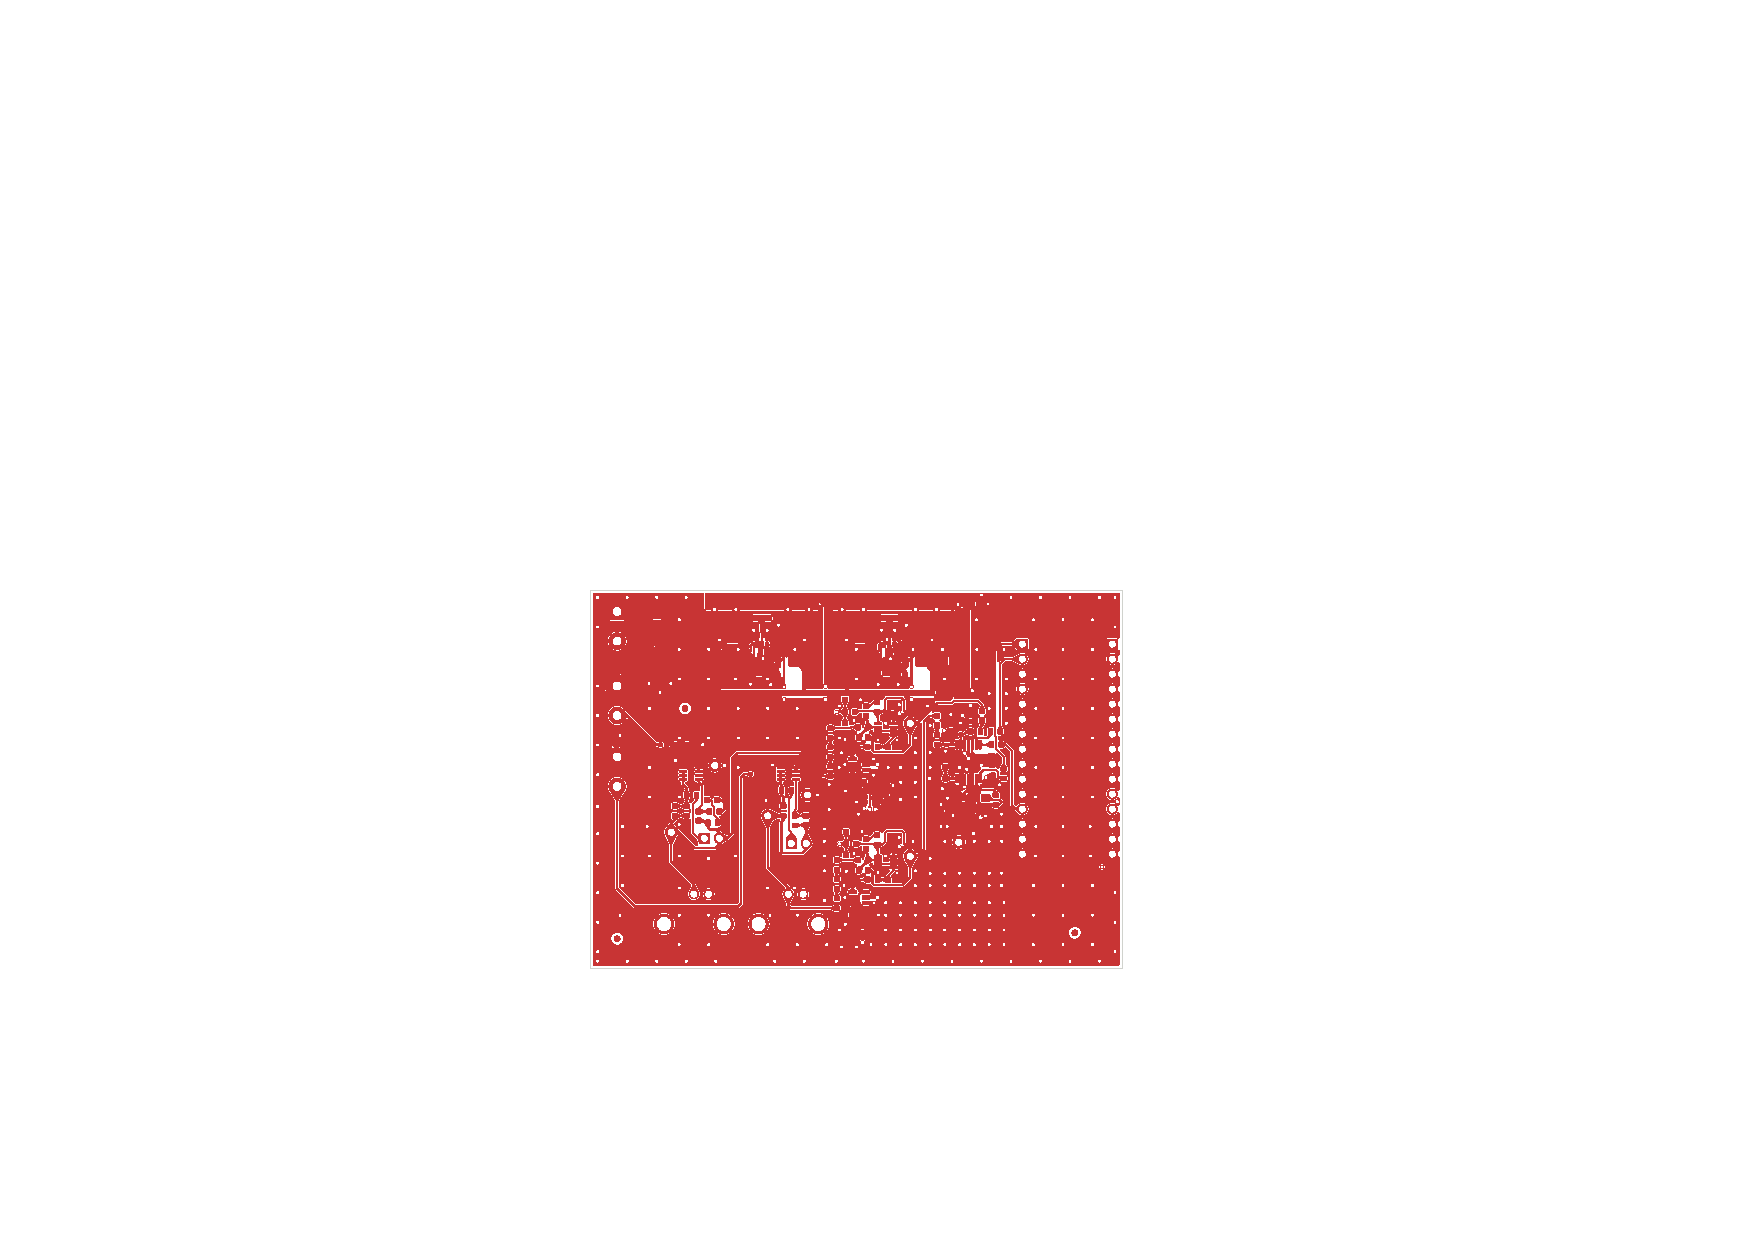
\includegraphics[width=0.47\linewidth]{figuras/capa_F_Cu.pdf} &
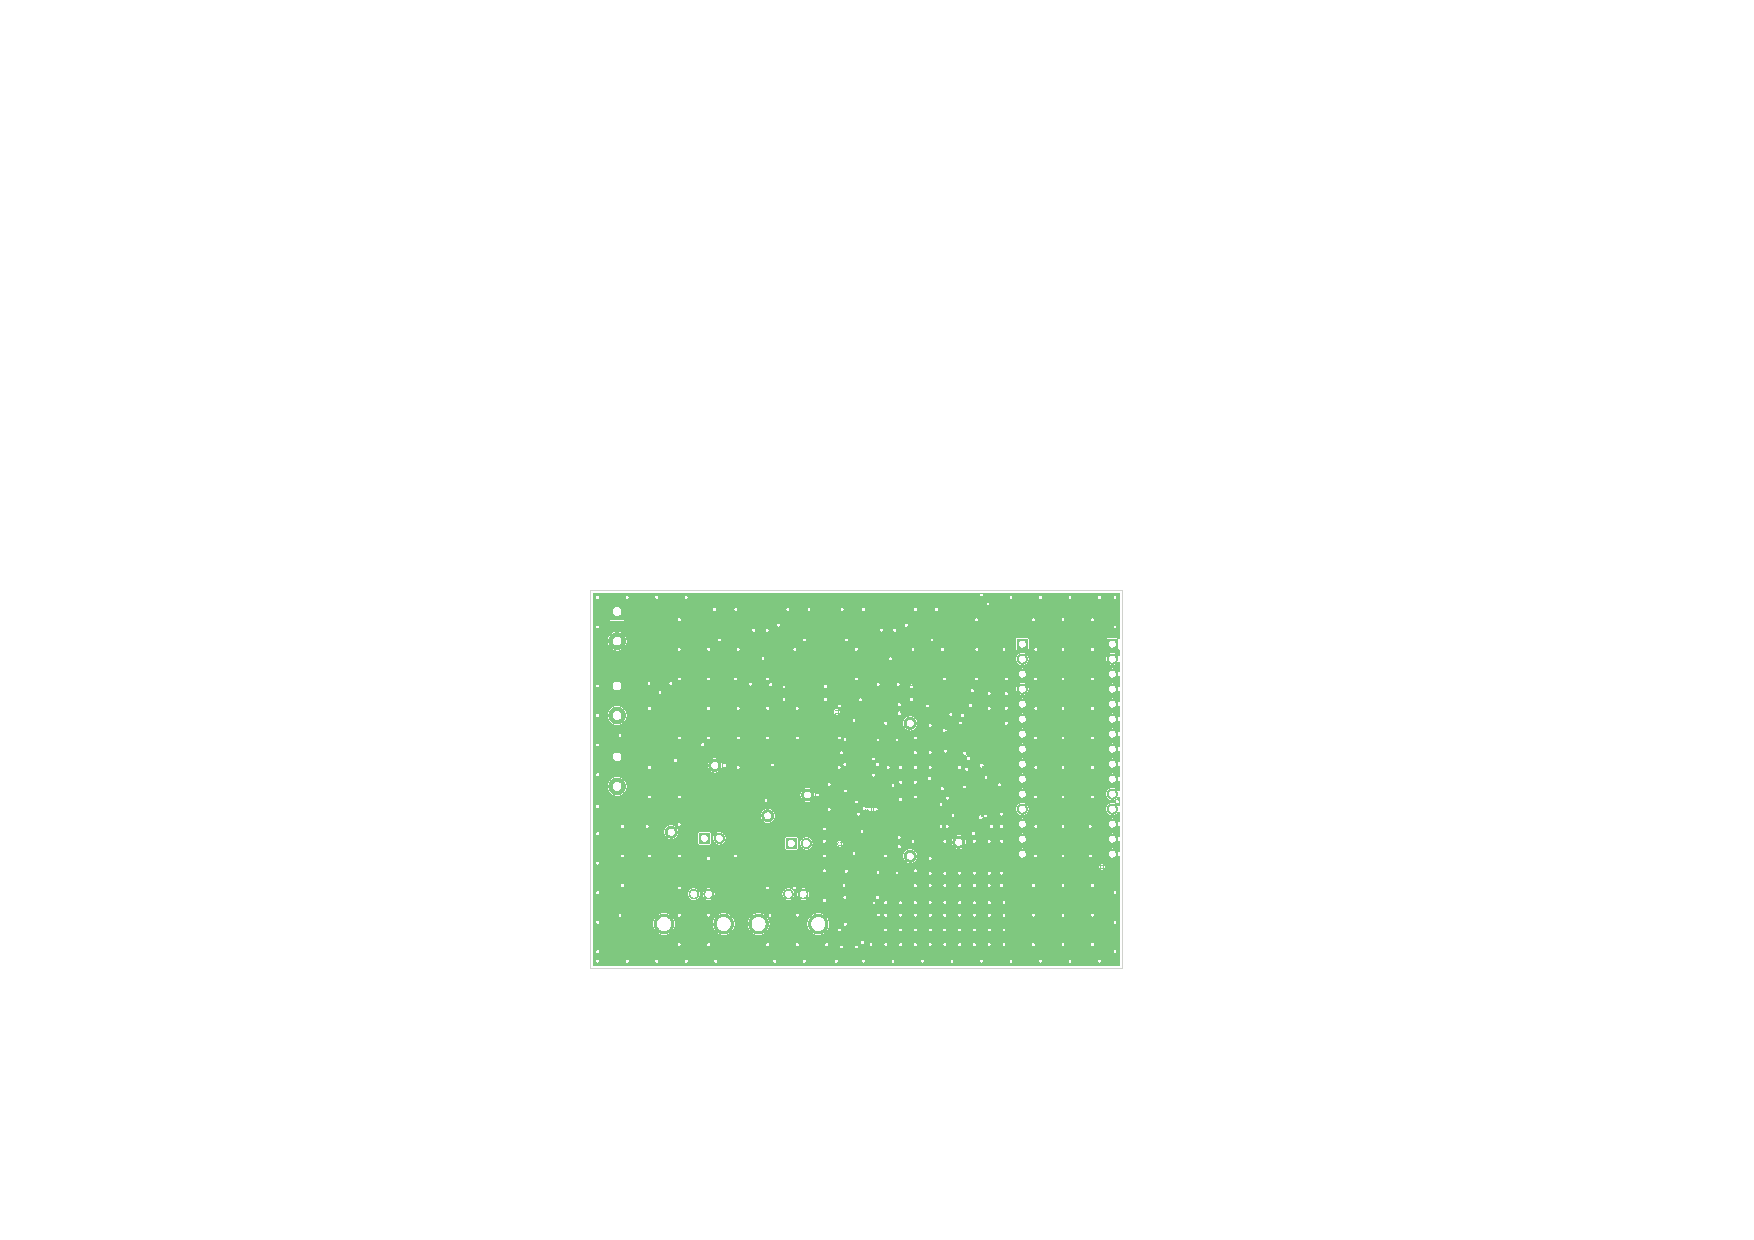
\includegraphics[width=0.47\linewidth]{figuras/capa_In1_Cu.pdf} \\
\small (a) \capa{F.Cu} & \small (b) \capa{In1.Cu} \\[3mm]
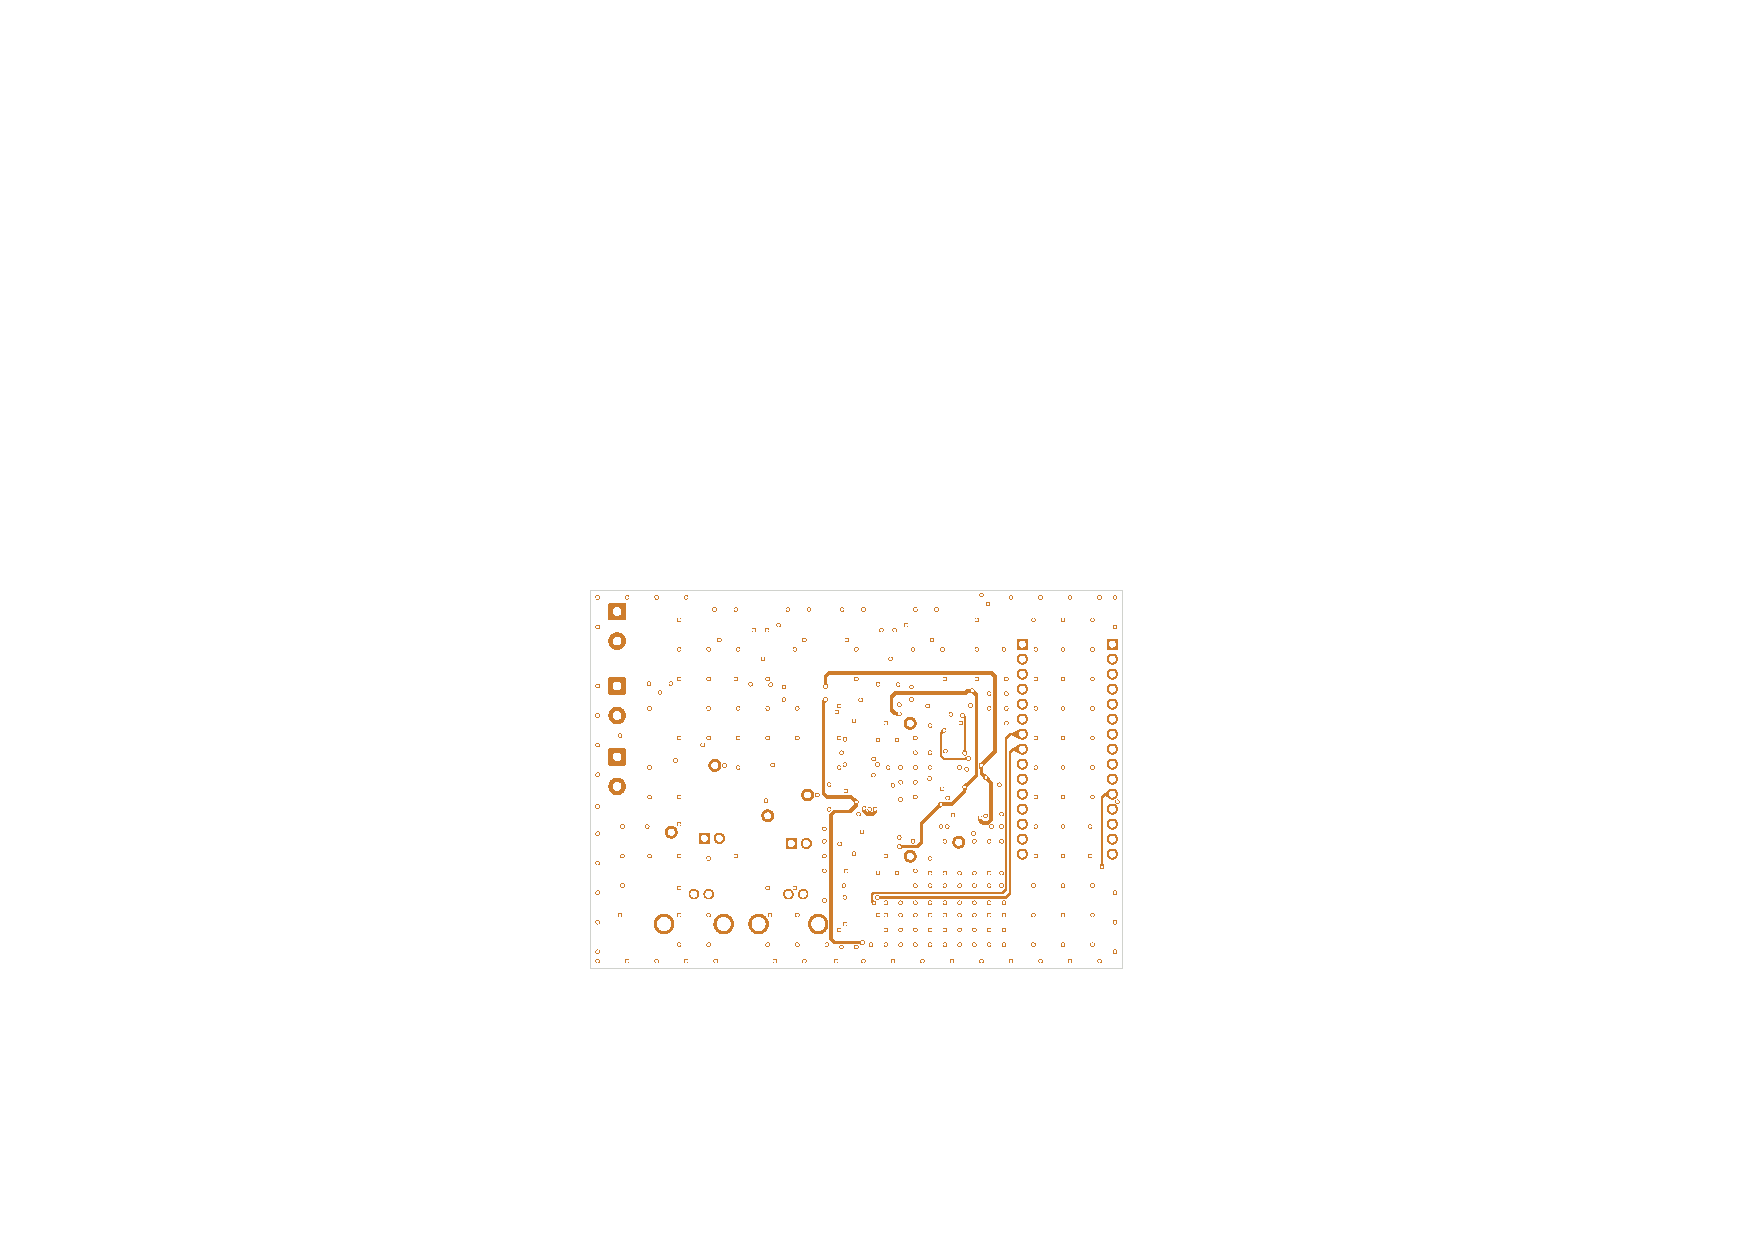
\includegraphics[width=0.47\linewidth]{figuras/capa_In2_Cu.pdf} &
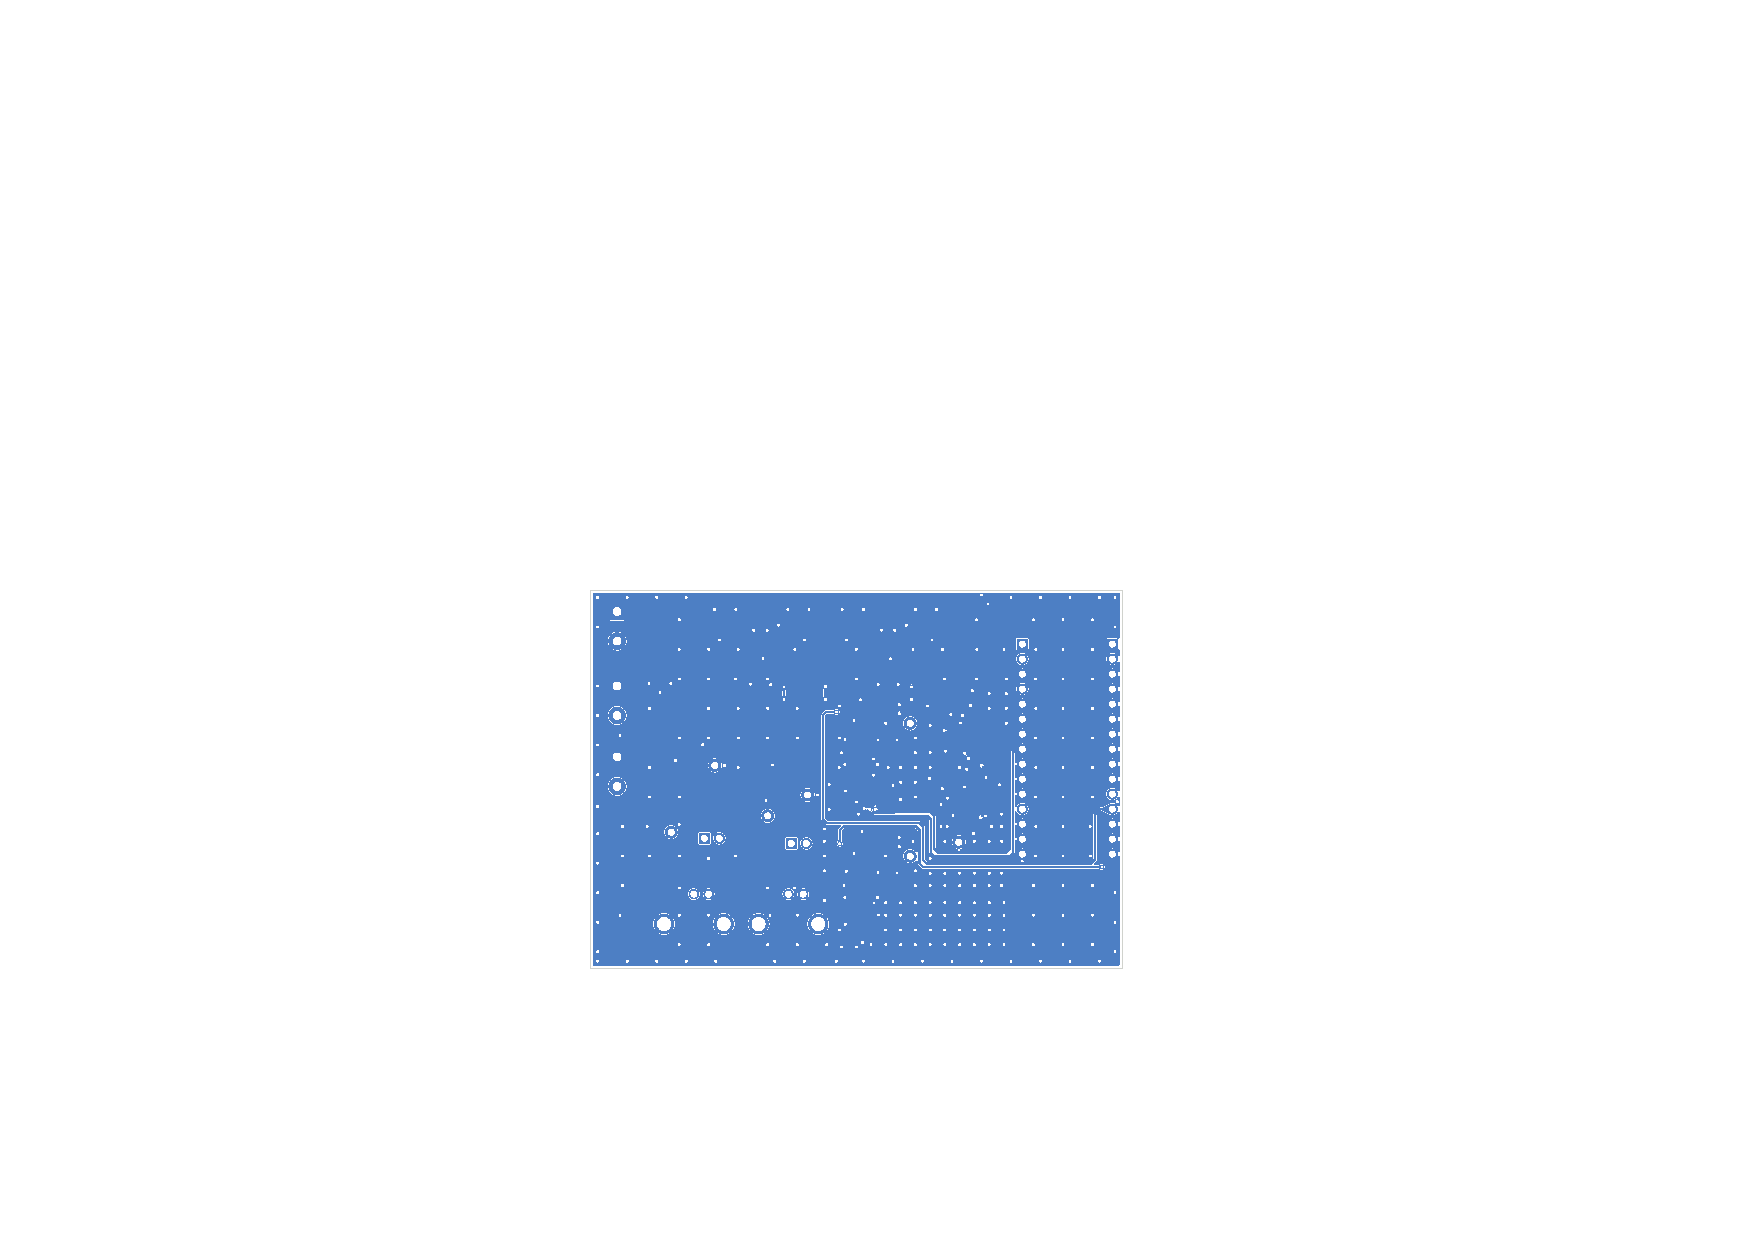
\includegraphics[width=0.47\linewidth]{figuras/capa_B_Cu.pdf} \\
\small (c) \capa{In2.Cu} & \small (d) \capa{B.Cu}
\end{tabular}
\caption{Las cuatro capas de cobre de la placa terminada (vista desde arriba, exportadas con \texttt{kicad-cli}).
(a) \capa{F.Cu}: casi todo es relleno GND; las pistas se ven como líneas blancas (las separaciones) y arriba están las
zonas de los dos buck. (b) \capa{In1.Cu}: plano GND entero; los puntos son las holguras de las vías y de los pines con
agujero. (c) \capa{In2.Cu}: solo pistas, sin plano: \net{3V3} y \net{5V_A} bajando desde los buck, y el I2C del canal 2
y \net{DC_MON2} llegando a la NUCLEO (columnas de pines a la derecha). (d) \capa{B.Cu}: zona GND con las pistas lentas
(I2C del canal 1, \net{DC_MON}, \net{DC_MON2}) recortadas en ella.}
\label{fig:c08-capas}
\end{figure}

% =====================================================================================================
\section{Cómo se verifica que se respete el uso de las capas}\label{sec:c08-politica}

Decidir el uso de cada capa no sirve de nada si no se comprueba. Se hizo con dos herramientas propias que leen la
placa con la API de KiCad (detalles en el capítulo~\ref{cap:verif}):

\begin{itemize}
  \item \textbf{Chequeo G de \archivo{revisar_pistas.py}:} \capa{In1.Cu} sin pistas (plano entero); las redes de clase
  Analógica, Reloj y Conmutado solo en \capa{F.Cu}, con dos excepciones: \net{DC_MON}/\net{DC_MON2} (son un nivel de
  DC filtrado) e \net{IEPE_FEED*} (el riel de \SI{24}{\volt} de cada fuente IEPE, que es DC). \capa{In2.Cu} y
  \capa{B.Cu} quedan para alimentación y señales lentas.
  \item \textbf{Chequeo I:} recorre cada pista crítica de \capa{F.Cu} y comprueba que debajo, en \capa{In1.Cu}, haya
  cobre GND continuo (contra el relleno real de la zona). Los únicos huecos permitidos son el anillo libre alrededor de
  un pad con agujero o de una vía de la misma red, justo donde la pista termina.
  \item \textbf{\archivo{cruces_capas.py}:} para cada pista de \capa{In2.Cu} y \capa{B.Cu} lista qué cobre de
  \capa{F.Cu} tiene encima. Marca como error si pasa debajo de un nodo protegido: los nodos \net{SUM}, el nodo filtrado
  del DAC, la cadena de \SI{1}{\mega\ohm} y el nodo medio de la realimentación. Resultado final: \textbf{0 cruces bajo
  nodos protegidos}; lo que queda encima de pistas de otras capas son \net{IEPE}, \net{REST_SV}, las líneas SAI y el
  I2C, todas de baja impedancia.
\end{itemize}

\begin{ojo}[por qué esta regla sigue valiendo con 4 capas]
Con \capa{In1.Cu} entero podrías pensar que ya da igual qué pase por \capa{In2.Cu} o \capa{B.Cu}. Para el retorno sí da
igual, porque el retorno de \capa{F.Cu} va por \capa{In1.Cu}, y el plano además hace de pantalla entre las capas. Pero
el plano no es perfecto: tiene holguras alrededor de cada vía y de cada pin con agujero. Con nodos de cientos de
k$\Omega$ (sección~\ref{sec:c08-altaz}) se prefirió no depender de eso, y la regla del dueño de los bloques 3 y 4 se
mantuvo. Respetarla no costó nada: el ruteo encontró camino para todas las redes lentas sin pasar bajo esos nodos.
\end{ojo}

% =====================================================================================================
\section{Cuánto cuesta y si sirve para el ensamblaje económico}\label{sec:c08-costo}

Cotización de JLCPCB sin sesión iniciada, sin envío ni ensamblaje, para 5 placas de \qtyproduct{90 x 64}{\milli\meter},
4 capas, \SI{1.6}{\milli\meter} y máscara verde \doc{REGLAS.md §9, cotizador JLCPCB, 2026-11-16}:

\begin{center}
\begin{tabular}{@{}lr@{}}
\toprule
\textbf{Acabado} & \textbf{Precio (5 placas)} \\
\midrule
HASL con plomo (oferta) & USD \num{8.00} \\
\textbf{HASL sin plomo (elegido)} & \textbf{USD \num{13.20}} \\
ENIG & USD \num{25.30} \\
\bottomrule
\end{tabular}
\end{center}

La versión de 2 capas de esta misma placa no se cotizó, así que no hay una diferencia de precio medida; las cifras de
blogs que se vieron al principio son de terceros y no se verificaron \copia. Lo que sí se comprobó es que el cambio no
saca a la placa del ensamblaje económico (\emph{Economic PCBA}): en la tabla de capacidades de JLCPCB, la fila de
Economic dice ``4L · 1.6 · Green · Lead-Free:HASL / ENIG · 2--50'' \doc{página de capacidades PCBA, 2026-11-16}, y la
misma página acepta 2, 4 y 6 capas, espesores de \SIrange{0.8}{1.6}{\milli\meter} y ``solo apilado estándar''.

\begin{ojo}[vías taponadas: una consecuencia directa de las 4 capas]
En placas de 4 capas JLCPCB tapona las vías por defecto (\emph{plugged}), y una vía a menos de \SI{0.35}{\milli\meter}
de un pad no se puede taponar con tinta \doc{JLCPCB, artículo de recubrimiento de vías}. Por eso, al pasar a 4 capas,
apareció una regla nueva (\texttt{via\_tapada\_lejos\_de\_pad}) y hubo que mover 43 vías ya puestas. Lo ves en el
capítulo~\ref{cap:ruteo}.
\end{ojo}

\section*{Resumen}
\begin{itemize}
  \item Toda señal forma un lazo con su retorno por tierra; a alta frecuencia el retorno va justo debajo de la pista, y
  el área del lazo decide cuánto ruido capta, emite y acopla.
  \item Un corte en el plano obliga al retorno a rodear y agranda el lazo. En 2 capas, cada pista en \capa{B.Cu} es un
  corte en el plano.
  \item Los nodos de la cadena de \SI{1}{\mega\ohm} tienen cientos de k$\Omega$: una capacidad parásita de
  \SI{0.1}{\pico\farad} ya deja pasar un 15\,\% de un ruido de \SI{1}{\mega\hertz}.
  \item La regla de 2 capas (plano en \capa{B.Cu}, críticas solo en \capa{F.Cu}) no tenía solución con el placement
  real: I2C y \net{DC_MON} nacen en los AFE y van a la NUCLEO cruzando una pared de señales críticas. El oráculo
  (Freerouting en copias) lo confirmó: 3 conexiones sin rutear aun usando \SI{140}{\milli\meter} de \capa{B.Cu} bajo
  12 redes críticas.
  \item Se eligió 4 capas: \capa{In1.Cu} es un plano GND entero a \SI{0.21}{\milli\meter} de \capa{F.Cu}, y las
  redes lentas se cruzan por \capa{In2.Cu} y \capa{B.Cu}. Resultado: cero excepciones de cruce y cero pistas bajo
  nodos protegidos.
  \item Cuesta USD \num{13.20} por 5 placas con HASL sin plomo y sigue siendo compatible con el ensamblaje económico de
  JLCPCB.
\end{itemize}
